\chapter{Analiza wymagań konkursu DAC SDC 2021}
\label{cha:Analiza probemu}

Opracowywany system powstaje na potrzeby konkursu \emph{Design Automation Conference System Design Contest 2021} (DAC SDC)
Rozpatrywanym problemem jest detekcja obiektów za pomocą sztucznej sieci neuronowej.
Realizacja zadania ma zostać przeprowadzona na wbudowanej platformie obliczeniowej typu \emph{SBC} (ang. \emph{Single Board Computer}).
W niniejszym rozdziale zostaną przedstawione założenia oraz wymagania stawiane wobec opracowywanego systemu detekcji.
Zostanie opisana docelowa platforma obliczeniowa. Zostaną przedstawione wybrane możliwe rozwiązania, 
a także dostępne narzędzia wspomagające docelową implementację.


\section{Wymagania}
Ze względu, iż opracowywany system powstaje na potrzeby konkursu, musi on spełniać stawiane założenia i wymagania.
Zadaniem jest detekcja siecią neuronową pojedynczych obiektów w sekwencjach zarejestrowanych podczas lotu drona.
Organizatorzy dostarczają zbiór treningowy składający się z obrazów o wymiarach 640 pikseli szerokości na 360 pikseli wysokości. Zbiór składa się z ponad 90 tysięcy obrazów, wchodzących w skład 95 sekwencji podzielonych na 12 kategorii. Na rysunku \ref{fig:sample_images} przedstawiono przykładowe obrazy znajdujące się w zbiorze uczącym wraz z zaznaczonymi obiektami detekcji.
\begin{figure}
    \centering
    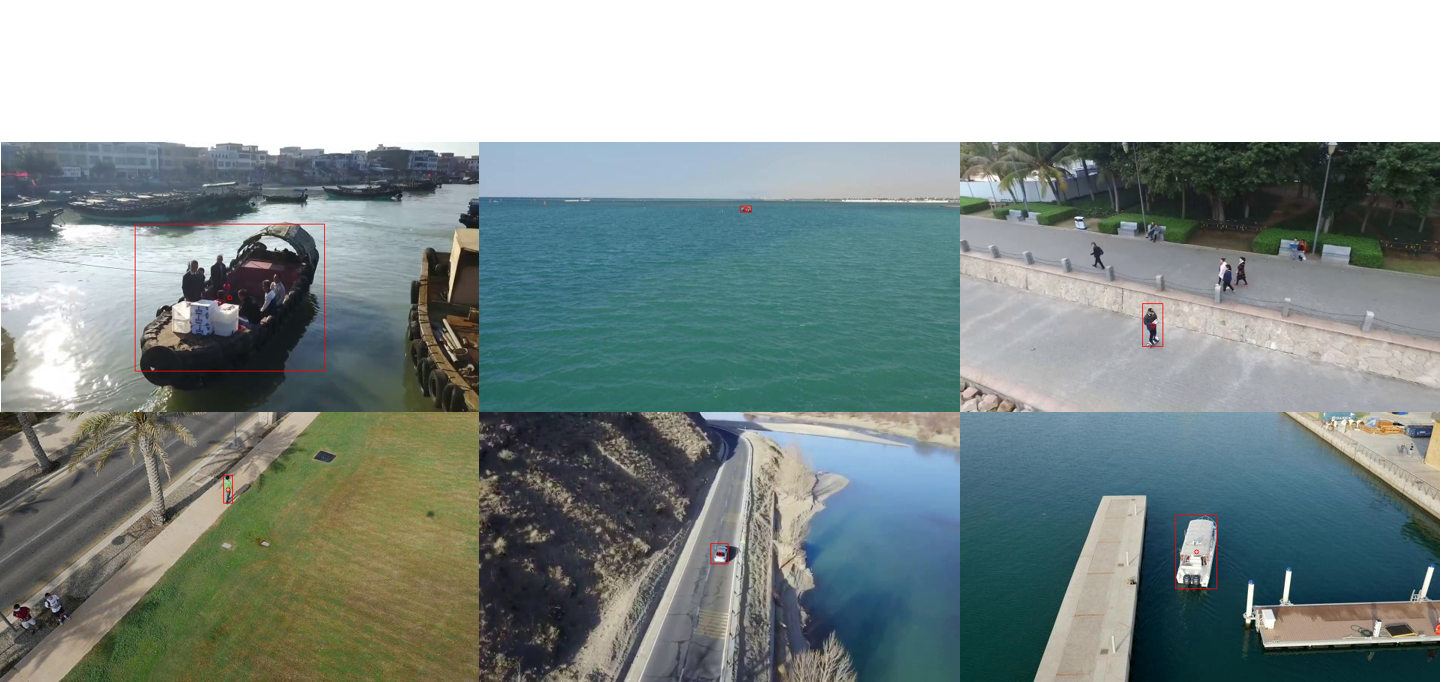
\includegraphics[width=\linewidth]{images/sample_images.png}
    \caption{Przykładowe obrazy zbioru uczącego wraz z zaznaczonymi obiektami detekcji. Źródło \cite{dac_sdc_2021}.}
    \label{fig:sample_images}
\end{figure}

Samo rozwiązanie poddawane jest ocenie danej wzorem \eqref{eq:score}. Uzyskanie wyższej wartości skutkuje uzyskaniem wyższego miejsca w rankingu, z czego wynika, iż funkcję $Score$ należy maksymalizować. 

\begin{equation}
E_{Score} = log_2(E)
\label{eq:e_score}
\end{equation}

\begin{equation}
IoU_{Score} = max(0.1, ReLU(1 - 5 ReLU(0.7 - IoU)))
\label{eq:iou_score}
\end{equation}

\begin{equation}
FPS_{Score} = ReLU(1 - ReLU( 1 - \frac{1}{FPS}))
\label{eq:fps_score}
\end{equation}

\begin{equation}
Score = \frac{10^2}{E_{Score}} IoU_{Score} FPS_{Score}
\label{eq:score}
\end{equation}

Ocenie poddawana jest zarówno dokładność detekcji mierzona współczynnikiem $IoU$ (ang. \emph{Intersection over Union}) na zbiorze tajnym, lecz również przepustowość $FPS$ mierzona poprzez liczbę przetworzonych obrazów na sekundę. 
Ponadto mierzona jest również całkowita energia $E$ zużyta przez układ. 
Zużyta energia jest wyznaczana z iloczynu zmierzonego czasu przetwarzania oraz pomiaru średniej mocy układu. 
Chwilowe wartości mocy są odczytywane z regulatora mocy z częstotliwością próbkowania $20 Hz$.
Zarówno pomiar energii oraz czasu musi być realizowany przez opracowaną aplikację.
Wstępna analiza pozwala stwierdzić, iż uzyskanie wartości $IoU$ oraz $FPS$ poniżej wartości progowych skutkuje zastosowanie kary, natomiast
%nadmierne 
zwiększanie tych wartość powyżej wartości progowych nie przynosi dodatkowych korzyści (przynajmniej w sposób bezpośredni). 

% Analizując wzór \eqref{eq:fps_score} można zauważyć, iż uzyskanie przepustowości powyżej $30 fps$ pozwala na osiągnięcie maksymalnej wartości współczynnika $FPS_{Score}$. Dalsze zwiększenie przepustowości nie zwiększa wartości $FPS_{Score}$. 
% Dla deterministycznego systemu wartość ta powinna być stała. Oczekiwane jest również, iż dla różnych egzemplarzy platformy wartości te będą przyjmowały zbliżoną wartość. Wówczas Funkcja oceny \eqref{eq:score} zależy jedynie od dokładności oraz zużycia energii.

Wśród wymagań znajdują się również informacje odnośnie dostarczenia wymaganych plików.
Aplikacja sterująca ma być zrealizowana w postaci notatnika \emph{Jupyter}.
Dodatkowo należy dostarczyć również pliki \emph{*.hwh} (plik opisu diagramu blokowego logiki programowalnej)
oraz \emph{*.bit} (plik konfiguracji logiki programowalnej) Ponadto należy dołączyć inne niezbędne pliki. 
Finalne rozwiązanie musi być dostępne w formie otwarto-źródłowej.

\section{Platforma sprzętowa}
Ewaluacja wytrenowanej sieci neuronowej jest przeprowadzana na wbudowanej platformie obliczeniowej \emph{Avnet Ultra96-V2} \cite{avnet_ultra96}. Jest to płytka rozwojowa wyposażona w układ \emph{Xilinx Zynq UltraScale+ MPSoC ZU3EG A484}, 2 GB pamięci LPDDR4, slot kart microSD, moduł Wi-Fi, a także porty USB 3.0, porty IO oraz port mini-display. Układ działa pod kontrolą systemu operacyjnego \emph{PetaLinux} wraz z uruchomionym serwerem \emph{Jupyter} (pochodzących z dystrybucji projektu \emph{Pynq}\cite{pynq}). 
Sam układ \emph{Xilinx Zynq UltraScale+ MPSoC ZU3EG A484} jest układem typu SoC. Zawiera czterordzeniowy procesor ARM Cortex-A53 MPCore, dwurdzeniowy procesor Arm Cortex-R5F MPCore oraz procesor graficzny Mali-400 MP2 \cite{zynq_product_guide}. Ponadto układ wyposażony jest w logikę programowalną połączoną z systemem procesorowym magistralą AXI. Logika programowalna zawiera: 154 tys. System Logic Cells, 141 tys. przerzutników oraz 71 tys. LUT (ang. Look-Up Table) zawartych w blokach CLB (ang. Configurable Logic Block), 360 DSP slice, a także 7.6 MB pamięci BRAM. Rysunek \ref{fig:ultra96} przedstawia docelową platformę.

\begin{figure}
    \centering
    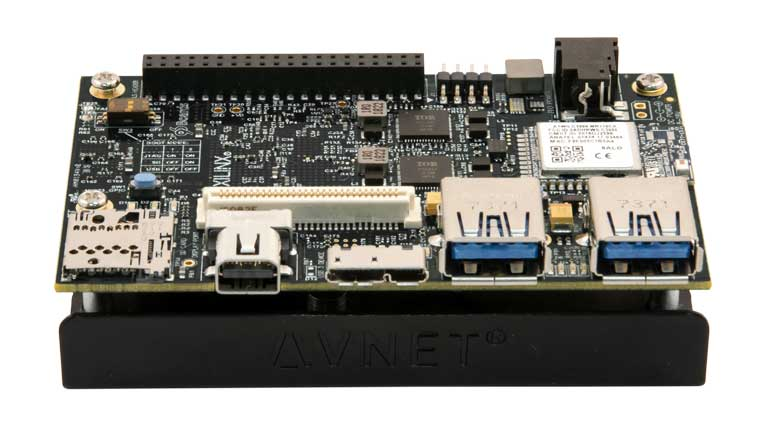
\includegraphics[width=\linewidth]{images/ultra96v2.png}
    \caption{Płytka \emph{Avnet Ultra96 V2}. Źródło \cite{avnet_ultra96}.}
    \label{fig:ultra96}
\end{figure}\section{Architektura wstępna}
 

\section{Przegląd rozwiązań}
Jednym z warunków konkursu jest udostępnienie pełnego rozwiązania w formie otwarto-źródłowej. 
Daje to możliwość analizy rozwiązań z edycji poprzedzających rozpatrywaną.

Zwycięski zespół poprzedniej edycji wykorzystał architekturę sieci \emph{Ultra\_net} \cite{ultra_net}. 
Architektura jest w pełni konwolucyjna (FCNN, ang. Fully Convloutional Neural Network), zawiera 9 warstw kowolucyjnych, warstwy normalizujące (przekształcenie afiniczne) oraz warstwy Max Pooling. 
Ponadto warstwy konwolucyjne zawierały co najwyżej 64 filtry (o wymiarze 3x3) i nie zawierały składowych stałych. Wyjątkiem jest ostatnia warstwa  stanowiąca warstwę typu \emph{YOLOv2}\cite{yolov2} / \emph{Yolov3}\cite{yolov3}, w której składowa stała występuje.
Sprzetowa akceleracja zostałą zrealizowana z użyciem języka HLS (ang. High Level Synthesis). 
Wykorzystano tutaj 4 bitową kwanytyzację wag konwolucji. 
Dla warstw normalizacyjnych kwantyzacja była różna (zależna od położenia warstwy).
Rozwiązanie osiągnęło dokładność detekcji $0.656$ IoU, przepustowość $212.726 fps$ oraz zużyło $1641.1 J$ energii. 

Innym rozwiązaniem jest architektura \emph{SkyNet}\cite{skynet}. 
Przez 3 ostatnie edycje architektura ta osiągała jedne z najlepszych wyników.
Jest to również sieć typu FCNN, wyróżniająca się zastosowaniem konwolucji seperowalnych oraz zastosowaniem funkcji aktywacji $ReLU6$.
W każdym bloku konwolucji separowalnej, po każdej warstwie konwolucji typu depthwise oraz pointwise  występuje warstwa normalizacji z funkcją aktywacji.
Ostatnią warstwę sieci stanowi warstwa \emph{YOLO} (podobnie jak w przypadku \emph{Ultra\_net}).
Ilość filtrów w warstwach oraz położenie warstw Max Pooling zostały zoptymalizowane z użyciem algorytmu PSO.
Rozwiązanie osiągnęło dokładność detekcji $0.716$ IoU, przepustowość $25.05 fps$ oraz zużyło $7260 J$ energii dla implementacji na płytce \emph{Avnet Ultra96 V1}. 

Dotychczas przytoczone rozwiązania wykorzystywały sieci z kwantyzacją wielobitową oraz pochodzące z poprzednich edycji konkursu. Innym podejściem mogącym uzyskać zwiększoną przepustowość oraz mniejsze zużycie energii jest zastosowanie sieci binarnych. Przykładem jest sieć \emph{XNOR-Net}\cite{xnor_net}. Wagi oraz wejścia warstw sieci są poddawane binaryzacji funkcją $sign$. 
Binarne wartości poddawane są binarnej konwolucji, która różni się względem standardowej użyciem funkcji $xor$ zamiast mnożenia. 
Celem poprawienia rezultatów treningu sieci oraz zmniejszenia różnicy pomiędzy odpowiedziami modelu zmiennoprzecinkowego wprowadzono współczynniki skalujące wyznaczane analitycznie. 
Następcą sieci \emph{XNOR-Net} jest sieć \emph{XNOR-Net++}\cite{xnor_net++}. W sieci tej zastąpiono wyznaczane analitycznie współczynniki na rzecz dodatkowych parametrów sieci wyznaczanych w trakcie wstecznej propagacji błędu.
Obie wspomniane sieci binarne były testowane przez autorów dla zadania klasyfikacji. 
Jednakże opisana metodyka może również być zastosowana dla zadania detekcji.


\section{Narzędzia}
Uzyskanie przepustowości $30 fps$, pozwalającej na uzyskanie wysokiej oceny rozwiązania, może być trudne lub nie możliwe do osiągnięcia przy użyciu jedynie części procesorowej nawet dla modeli o niskiej złożoności obliczeniowej. 
Wymagana jest tutaj dodatkowa akceleracja wykorzystująca logikę programowalną. 
W tym celu możliwe jest wykorzystanie istniejących narzędzi wspomagających sprzętową implementację, a także proces uczenia. 

Uczenie sieci z przeznaczeniem do sprzętowej akceleracji zazwyczaj wiąże się z wytrenowaniem modelu zmiennoprzecinkowego, następnie jego kwantyzacji oraz finalnie implementacji sprzętowej.
Etap wytrenowania modelu zmiennoprzecinkowego może zostać przeprowadzony z użyciem dowolnych narzędzi, narzędzi wspieranych na dalszych etapach lub konwersji modelu do wspieranego formatu. 
Następnym etapem jest kwantyzacja. Na tym etapie wagi oraz wyniki pośrednie warstw sieci są poddawane kwantyzacji. 
Zazwyczaj wyniki sieci kwantyzowanej różnią się od wyników modelu zmiennoprzecinkowego, przez co wymagane jest wznowienie procesu uczenia.
Daje to możliwość pominięcia treningu modelu zmiennoprzecinkowego.
Model kwantyzowany możliwy jest do sprzętowej implementacji z wykorzystaniem wybranych narzędzi.

Poniżej wymieniono wybrane narzędzia wspomagające sprzętową implementację. 
\begin{itemize}
    \item \emph{Brevitas}\cite{brevitas} - biblioteka dla frameworka \emph{PyTorch}\cite{pytorch}, przeznaczona do wspomagania kwantyzacji i treningu QNN. Biblioteka rozwijana przez \emph{Xilinx}.
    
    \item \emph{FINN}\cite{finn} - framework rozwijany przez \emph{Xilinx} pozwalający na implementację sprzętową QNN w typie przetwarzania potokowego.
    
    \item \emph{QKeras}\cite{qkeras} - biblioteka dla frameworka \emph{TensorFlow}\cite{tf} pozwalająca na kwantyzację i trening QNN.
    \item \emph{hls4ml}\cite{hls4ml} - biblioteka dokonująca konwersji modelu QNN do zapisu z użyciem języka HLS. 
    
    \item \emph{Vitis AI}\cite{vitis_ai} - środowisko pozwalające na przeprowadzenie kwantyzacji, optymalizacji architektury sieci oraz sterowania procesem akceleracji poprzez stosowne biblioteki C++/Python. Jest to środowisko rozwijane przez firmę \emph{Xilinx}
    Wykorzystywana jest tutaj akceleracja z wykorzystaniem generycznego DPU (ang. Deep Processing Unit) możliwego do konfiguracji.
    
\end{itemize}


W analizę problemu włączono zarówno wymagania konkursowe, dostępną platformę sprzętową, a także istniejące rozwiązania i narzędzia.
Głównym celem jest implementacja szybkiego i energooszczędnego rozwiązania, pozwalającego na dokładną detekcję pojedynczych obiektów. 
Zadanie jest realizowane w oparciu o sprzętową akcelerację wykorzystującą logikę programowalną płytki \emph{Avnet Ultra96 V2}.
Dostępnych jest wiele bibliotek usprawniających proces kwantyzacji, jak również implementacji sprzętowej.
Możliwe jest wykorzystanie lub wzorowanie się na istniejących już rozwiązaniach zapewniających wysoką przepustowość oraz niskie zużycie energii. 


% Należy zaznaczyć, iż architektury sieci przed i po procesie kwantyzacji nie mogą lub nie powinny być rozważanie jako identyczne ze względu na znaczne zmiany jakie wprowadza kwantyzacja.  


%---------------------------------------------------------------------------

    

